\section{Results}
\label{results}
In this section I will discuss the balancing results for the two main algorithms I tested the pass on: RC4 and AES.
Both algorithms have been written/adapted so that they utilize the stack as much as possible, maximizing the benefits of my balancing pass.
For the evaluation of both the performance and the robustness I use histograms of the \hammingw{}s over the entire execution of the code.
\Cref{fig:rc4,fig:aes} show a comparison of balanced and unbalanced histograms for RC4 and AES respectively.

The balanced version of both algorithms have been compiled with my balancing pass, while the unbalanced versions were compiled with \crossgcc.

\begin{figure}[hp]
  \centering
  \begin{subfigure}[b]{0.49\textwidth}
    \begin{tikzpicture}
\begin{axis}[
    ybar,
    bar width=0.015\textwidth,
    enlargelimits=0.05,
    xtick={0,8,16,24,32},
    width=\textwidth,
]
\addplot[pantone289,fill=pantone289!40] table [x=i, y=unbalanced-total, col sep=comma] {data/rc4.csv};
\end{axis}
\end{tikzpicture}

    \caption{Unbalanced RC4}
  \end{subfigure}
  \begin{subfigure}[b]{0.49\textwidth}
    % This file was created by matplotlib2tikz v0.7.4.
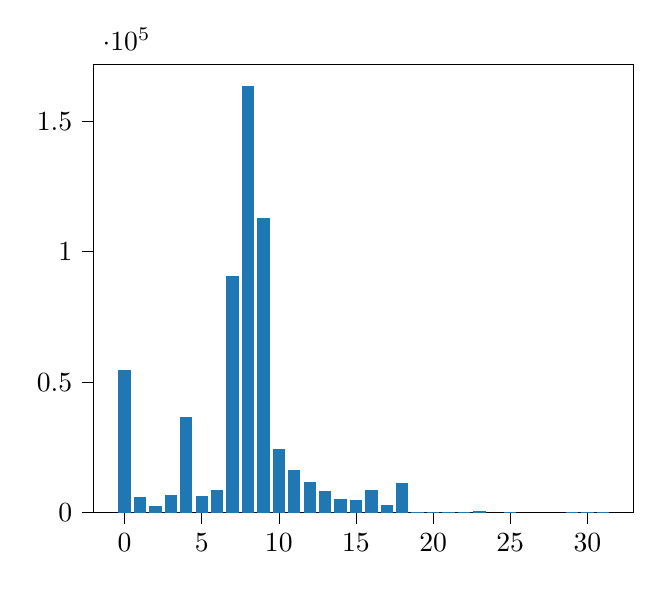
\begin{tikzpicture}

\definecolor{color0}{rgb}{0.12156862745098,0.466666666666667,0.705882352941177}

\begin{axis}[
tick align=outside,
tick pos=left,
x grid style={white!69.01960784313725!black},
xmin=-1.99, xmax=32.99,
xtick style={color=black},
y grid style={white!69.01960784313725!black},
ymin=0, ymax=171938.55,
ytick style={color=black}
]
\draw[fill=color0,draw opacity=0] (axis cs:-0.4,0) rectangle (axis cs:0.4,54571);
\draw[fill=color0,draw opacity=0] (axis cs:0.6,0) rectangle (axis cs:1.4,6050);
\draw[fill=color0,draw opacity=0] (axis cs:1.6,0) rectangle (axis cs:2.4,2313);
\draw[fill=color0,draw opacity=0] (axis cs:2.6,0) rectangle (axis cs:3.4,6824);
\draw[fill=color0,draw opacity=0] (axis cs:3.6,0) rectangle (axis cs:4.4,36773);
\draw[fill=color0,draw opacity=0] (axis cs:4.6,0) rectangle (axis cs:5.4,6353);
\draw[fill=color0,draw opacity=0] (axis cs:5.6,0) rectangle (axis cs:6.4,8761);
\draw[fill=color0,draw opacity=0] (axis cs:6.6,0) rectangle (axis cs:7.4,90865);
\draw[fill=color0,draw opacity=0] (axis cs:7.6,0) rectangle (axis cs:8.4,163751);
\draw[fill=color0,draw opacity=0] (axis cs:8.6,0) rectangle (axis cs:9.4,112999);
\draw[fill=color0,draw opacity=0] (axis cs:9.6,0) rectangle (axis cs:10.4,24463);
\draw[fill=color0,draw opacity=0] (axis cs:10.6,0) rectangle (axis cs:11.4,16480);
\draw[fill=color0,draw opacity=0] (axis cs:11.6,0) rectangle (axis cs:12.4,11631);
\draw[fill=color0,draw opacity=0] (axis cs:12.6,0) rectangle (axis cs:13.4,8125);
\draw[fill=color0,draw opacity=0] (axis cs:13.6,0) rectangle (axis cs:14.4,5158);
\draw[fill=color0,draw opacity=0] (axis cs:14.6,0) rectangle (axis cs:15.4,4929);
\draw[fill=color0,draw opacity=0] (axis cs:15.6,0) rectangle (axis cs:16.4,8458);
\draw[fill=color0,draw opacity=0] (axis cs:16.6,0) rectangle (axis cs:17.4,2812);
\draw[fill=color0,draw opacity=0] (axis cs:17.6,0) rectangle (axis cs:18.4,11488);
\draw[fill=color0,draw opacity=0] (axis cs:18.6,0) rectangle (axis cs:19.4,374);
\draw[fill=color0,draw opacity=0] (axis cs:19.6,0) rectangle (axis cs:20.4,342);
\draw[fill=color0,draw opacity=0] (axis cs:20.6,0) rectangle (axis cs:21.4,206);
\draw[fill=color0,draw opacity=0] (axis cs:21.6,0) rectangle (axis cs:22.4,170);
\draw[fill=color0,draw opacity=0] (axis cs:22.6,0) rectangle (axis cs:23.4,456);
\draw[fill=color0,draw opacity=0] (axis cs:23.6,0) rectangle (axis cs:24.4,0);
\draw[fill=color0,draw opacity=0] (axis cs:24.6,0) rectangle (axis cs:25.4,179);
\draw[fill=color0,draw opacity=0] (axis cs:25.6,0) rectangle (axis cs:26.4,0);
\draw[fill=color0,draw opacity=0] (axis cs:26.6,0) rectangle (axis cs:27.4,0);
\draw[fill=color0,draw opacity=0] (axis cs:27.6,0) rectangle (axis cs:28.4,2);
\draw[fill=color0,draw opacity=0] (axis cs:28.6,0) rectangle (axis cs:29.4,8);
\draw[fill=color0,draw opacity=0] (axis cs:29.6,0) rectangle (axis cs:30.4,41);
\draw[fill=color0,draw opacity=0] (axis cs:30.6,0) rectangle (axis cs:31.4,16);
\end{axis}

\end{tikzpicture}

    \caption{Balanced RC4}
  \end{subfigure}

  \begin{subfigure}[b]{\textwidth}
    % This file was created by matplotlib2tikz v0.7.4.
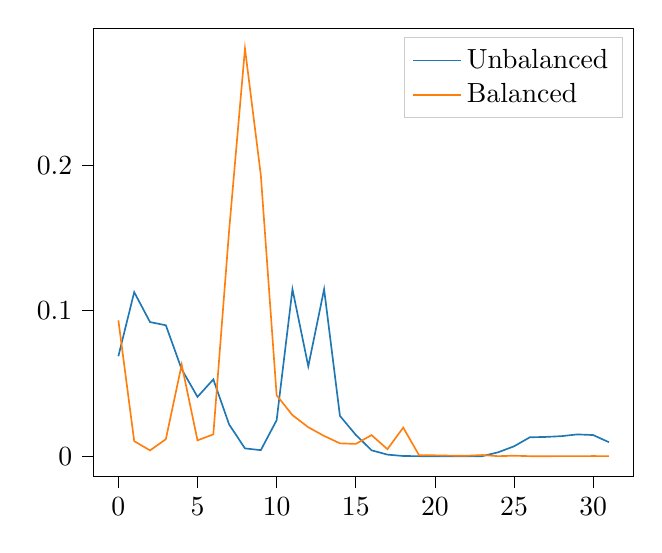
\begin{tikzpicture}

\definecolor{color0}{rgb}{0.12156862745098,0.466666666666667,0.705882352941177}
\definecolor{color1}{rgb}{1,0.498039215686275,0.0549019607843137}

\begin{axis}[
legend cell align={left},
legend style={draw=white!80.0!black},
tick align=outside,
tick pos=left,
x grid style={white!69.01960784313725!black},
xmin=-1.55, xmax=32.55,
xtick style={color=black},
y grid style={white!69.01960784313725!black},
ymin=-0.0140054362142874, ymax=0.294114160500036,
ytick style={color=black}
]
\addplot [semithick, color0]
table {%
0 0.0686886708296164
1 0.112735781975203
2 0.0921666731308743
3 0.0899559141036083
4 0.0597292789822751
5 0.0407632936430982
6 0.0527737915163738
7 0.0217455946424647
8 0.0053394355453852
9 0.00412416450115709
10 0.0247062017608502
11 0.114713829525915
12 0.0617719686098075
13 0.114752614772007
14 0.0276926657099639
15 0.014647894607558
16 0.00403366559360819
17 0.00106013005985856
18 0.000116355738277159
19 0
20 0
21 0
22 0
23 0
24 0.00268911039573879
25 0.0067744896508035
26 0.0129801290255853
27 0.0132257689175038
28 0.0137558339474331
29 0.014958176576297
30 0.0145186104539167
31 0.00957995578481946
};
\addlegendentry{Unbalanced}
\addplot [semithick, color1]
table {%
0 0.0933479074509321
1 0.0103489919568661
2 0.00395656502417046
3 0.0116729786964718
4 0.0629030547487333
5 0.0108672968433009
6 0.0149863666998519
7 0.155431595729031
8 0.280108724285749
9 0.193293511096514
10 0.041845849626581
11 0.0281903119750666
12 0.0198957232149272
13 0.0138984396114937
14 0.00882315710967195
15 0.00843143493477569
16 0.0144680618134171
17 0.00481014303846404
18 0.0196511106777649
19 0.000639755866424449
20 0.000585017396569951
21 0.000352378899688333
22 0.000290798121102022
23 0.000780023195426601
24 0
25 0.0003061933157486
26 0
27 0
28 3.42115436590614e-06
29 1.36846174636246e-05
30 7.0133664501076e-05
31 2.73692349272492e-05
};
\addlegendentry{Balanced}
\end{axis}

\end{tikzpicture}
    \caption{Scaled Hamming weight histograms for RC4}
  \end{subfigure}
  \caption{Hamming weight histograms for balanced and unbalanced RC4}
  \label{fig:rc4}
\end{figure}

\begin{figure}[hp]
  \centering
  \begin{subfigure}[b]{0.49\textwidth}
    \begin{tikzpicture}
\begin{axis}[
    ybar,
    bar width=0.015\textwidth,
    enlargelimits=0.05,
    xtick={0,8,16,24,32},
    width=\textwidth,
]
\addplot[pantone289,fill=pantone289!40] table [x=i, y=unbalanced-total, col sep=comma] {data/aes.csv};
\end{axis}
\end{tikzpicture}

    \caption{Unbalanced AES}
  \end{subfigure}
  \begin{subfigure}[b]{0.49\textwidth}
    \begin{tikzpicture}
\begin{axis}[
    ybar,
    bar width=0.015\textwidth,
    enlargelimits=0.05,
    xtick={0,8,16,24,32},
    width=\textwidth,
    xlabel={\hammingw{}},
    ylabel={Occurences}
]
\addplot[pantone289,fill=pantone289!40] table [x=i, y=balanced-total, col sep=comma] {data/aes.csv};
\end{axis}
\end{tikzpicture}

    \caption{Balanced AES}
  \end{subfigure}

  \begin{subfigure}[b]{\textwidth}
    \begin{tikzpicture}
\begin{axis}[
    ybar=2*\pgflinewidth,
    bar width=0.00725\textwidth,
    enlargelimits=0.05,
    xtick={0,8,16,24,32},
    width=\textwidth
]
\addplot[pantone289,fill=pantone289!40] table [x=i, y=unbalanced-scaled, col sep=comma] {data/aes.csv};
\addplot[pantone144,fill=pantone144!40] table [x=i, y=balanced-scaled, col sep=comma] {data/aes.csv};
\end{axis}
\end{tikzpicture}

    \caption{Scaled Hamming weight histograms for AES}
  \end{subfigure}
  \caption{Hamming weight histograms for balanced and unbalanced AES}
  \label{fig:aes}
\end{figure}

\subsection{Robustness}
For both algorithm the balancig works very well.
The \hammingw{}s are concentrated around 8, with other values being much less frequent.
Note that for an attacker performing Power Analysis, all values with the same \hammingw{} look the same.
Thus, the less evenly distributed the \hammingw{}s of intermediate values are, the lower the confidence of her statistical attack.
As such, a perfect scenario for the defender would be all \hammingw{}s having exactly the same value.

A significant number of operations also exhibit a \hammingw{} of 9 and 10, which is probably due to carry bits in arithmetic operations.
This theory is supported by the fact that these \hammingw{}s are more prevalent in AES, which utilizes a lot more loops and therefore additions.

The balancing is not perfect, as some intermediate steps of my balanced operators will \emph{always} have unbalanced values.
Value unbalancing for array indexing is also a factor for the distribution of \hammingw{}s in the balanced code.

\subsection{Performance}
The number of operations is $77349$ for unbalanced RC4, and $584598$ for balanced RC4.
That is an increase in the number of operations by a factor of $7.56$.

For AES the unbalanced code has $83549$ operations, while the balanced code has $2873960$ operations.
This is an increase by a factor of $34.4$.
The performance impact for AES can be reduced to a factor of $28.51$ when directly computing multiplication, which drops the number of operations to $2382048$.

For both algorithms the largest part of the performance impact is probably due to MUL, DIV and REM operations being calculated via repeated addition/subtraction.

In general it is also important to note that when the full 32bit range is required for the program the performance drops by an additional factor of 4, because then every operation needs to be performed on the individual bytes of a 32bit word.
This is less true for cryptographic algorithms, as they mostly work on individual bytes.
